\chapter{Dynaaminen ohjelmointi}

Dynaaminen ohjelmointi on tekniikka,
jonka avulla voimme ratkaista tehokkaasti monia
algoritmiikan ongelmia.
Ideana on muotoilla ongelma rekursiivisesti niin,
että ratkaisu ongelmaan palautuu saman ongelman
pienempiin osaongelmiin.
Tämän jälkeen saamme aikaan tehokkaan ratkaisun,
kun laskemme jokaisen osaongelman ratkaisun vain kerran.

Tässä luvussa tutustumme ensin dynaamisen ohjelmoinnin perusteisiin
käyttäen esimerkkinä tehtävää, jossa rakennamme torneja palikoista.
Tämän jälkeen käymme läpi kokoelman muita tehtäviä, jotka esittelevät
lisää dynaamisen ohjelmoinnin mahdollisuuksia.

\section{Perustekniikat}

Aloitamme dynaamiseen ohjelmointiin tutustumisen
seuraavasta tehtävästä:
meillä on palikoita, joiden korkeudet ovat 1, 2 ja 3,
ja haluamme rakentaa niistä tornin, jonka korkeus on $n$.
Jokaista palikkatyyppiä on saatavilla rajattomasti.
Monellako tavalla voimme rakentaa tornin?

\begin{figure}
\center
\begin{tikzpicture}[scale=0.7]
\newcommand\palikka[3]{
\draw (2*#1,#2) rectangle (2*#1+1,#2+#3);
}
\palikka{0}{0}{1} \palikka{0}{1}{1} \palikka{0}{2}{1} \palikka{0}{3}{1}
\palikka{1}{0}{1} \palikka{1}{1}{1} \palikka{1}{2}{2}
\palikka{2}{0}{1} \palikka{2}{1}{2} \palikka{2}{3}{1}
\palikka{3}{0}{2} \palikka{3}{2}{1} \palikka{3}{3}{1}
\palikka{4}{0}{2} \palikka{4}{2}{2}
\palikka{5}{0}{1} \palikka{5}{1}{3}
\palikka{6}{0}{3} \palikka{6}{3}{1}
\end{tikzpicture}
\caption{Voimme rakentaa korkeuden 4 tornin 7 tavalla palikoista,
joiden korkeudet ovat 1, 2 ja 3.}
\label{fig:dyntor}
\end{figure}

Kuva \ref{fig:dyntor} näyttää esimerkin, jossa $n=4$
ja meillä on 7 tapaa rakentaa torni palikoista.
Jos $n$ on pieni, voimme laskea tornien määrän helposti
käymällä läpi kaikki tavat, mutta tornien määrä kasvaa
nopeasti emmekä voi käyttää raakaa voimaa suuremmilla
$n$:n arvoilla.
Seuraavaksi ratkaisemmekin ongelman tehokkaasti
dynaamisen ohjelmoinnin avulla.

\subsection{Rekursiivinen esitys}

Jotta voimme käyttää dynaamista ohjelmointia,
meidän täytyy pystyä esit\-tämään ongelma rekursiivisesti
niin, että saamme laskettua ongelman ratkaisun
käyttäen osaongelmina pienempiä vastaavia ongelmia.
Tässä tehtävässä luonteva rekursiivinen funktio on
$\texttt{tornit}(n)$: monellako tavalla voimme
rakentaa tornin, jonka korkeus on $n$?
Esimerkiksi $\texttt{tornit}(4)=7$, koska
voimme rakentaa korkeuden 4 tornin 7 tavalla.

Funktion pienten arvojen laskeminen on helppoa.
Ensinnäkin $\texttt{tornit}(0)=1$, koska voimme
muodostaa tyhjän tornin yhdellä tavalla:
siinä ei ole mitään palikoita.
Sitten $\texttt{tornit}(1)=1$, koska ainoa mahdollisuus
rakentaa torni on valita korkeuden 1 palikka,
ja $\texttt{tornit}(2)=2$, koska voimme joko valita
kaksi korkeuden 1 palikkaa tai yhden korkeuden 2 palikan.

\begin{figure}
\center
\begin{tikzpicture}[scale=0.7]
\draw (0,0) rectangle (1,1);
\draw[dashed] (0,1) rectangle (1,4);
\draw (4,0) rectangle (5,2);
\draw[dashed] (4,2) rectangle (5,4);
\draw (8,0) rectangle (9,3);
\draw[dashed] (8,3) rectangle (9,4);
\draw [decorate,decoration={brace,amplitude=4pt},xshift=0.2cm] (1,4) -- (1,1) node [midway,right,xshift=.1cm] {$n-1$};
\draw [decorate,decoration={brace,amplitude=4pt},xshift=0.2cm] (5,4) -- (5,2) node [midway,right,xshift=.1cm] {$n-2$};
\draw [decorate,decoration={brace,amplitude=4pt},xshift=0.2cm] (9,4) -- (9,3) node [midway,right,xshift=.1cm] {$n-3$};
\end{tikzpicture}
\caption{Rekursiivinen idea: kun alamme rakentaa tornia, voimme laittaa pohjalle
korkeuden 1, 2 tai 3 palikan.}
\label{fig:dynrek}
\end{figure}

Kuinka voisimme sitten laskea funktion arvon yleisessä tapauksessa,
kun tornin korkeus on $n$?
Tässä voimme miettiä, kuinka tornin rakentaminen alkaa.
Meillä on kolme mahdollisuutta: voimme laittaa ensin palikan
korkeutta 1, 2 tai 3.
Jos valitsemme korkeuden 1 palikan, meidän täytyy rakentaa
sen päälle korkeuden $n-1$ torni.
Vastaavasti jos valitsemme korkeuden 2 tai 3 palikan,
meidän täytyy rakentaa sen päälle torni,
jonka korkeus on $n-2$ tai $n-3$.
Kuva \ref{fig:dynrek} havainnollistaa tämän idean.

Niinpä voimme laskea tornien määrän rekursiivisesti kaavalla
\[
\texttt{tornit}(n) = \texttt{tornit}(n-1)+\texttt{tornit}(n-2)+\texttt{tornit}(n-3),
\]
kun $n \ge 3$.
Esimerkiksi voimme laskea
\[
\texttt{tornit}(3) = \texttt{tornit}(2)+\texttt{tornit}(1)+\texttt{tornit}(0)=4
\]
ja
\[
\texttt{tornit}(4) = \texttt{tornit}(3)+\texttt{tornit}(2)+\texttt{tornit}(1)=7,
\]
jolloin olemme saaneet laskettua esimerkkitapaustamme vastaavasti,
että voimme rakentaa korkeuden 4 tornin 7 tavalla.

\begin{table}
\center
\begin{tabular}{rrr}
korkeus $n$ & $\texttt{tornit}(n)$ \\
\hline
0 & 1 \\
1 & 1 \\
2 & 2 \\
3 & 4 \\
4 & 7 \\
5 & 13 \\
6 & 24 \\
7 & 44 \\
8 & 81 \\
9 & 149 \\
\end{tabular}
\caption{Tornien määrät, kun korkeus $n$ on $0,1,\dots,9$.}
\label{tab:dyntor}
\end{table}

Taulukko \ref{tab:dyntor} näyttää yhteenvedon funktion
$\texttt{tornit}(n)$ arvoista, kun $n=0,1,\dots,9$.
Kuten taulukosta voi huomata, funktion arvo kasvaa nopeasti:
se lähes kaksinkertaistuu joka askeleella.
Kun $n$ on suuri,
meillä onkin valtavasti mahdollisuuksia tornin rakentamiseen.

\subsection{Tehokas toteutus}

Nyt kun olemme saaneet aikaan rekursiivisen funktion,
voimme toteuttaa sen ohjelmoimalla seuraavasti:

\begin{code}
function tornit(n)
    if (n == 0) return 1
    if (n == 1) return 1
    if (n == 2) return 2
    return tornit(n-1)+tornit(n-2)+tornit(n-3)
\end{code}

Tämä on toimiva ratkaisu, mutta siinä on yksi ongelma:
funktion arvon laskeminen vie kauan aikaa, jos $n$ on
vähänkin suurempi.
Käytännössä laskenta alkaa hidastua parametrin $n=30$ tienoilla.
Esimerkiksi arvon $\texttt{tornit}(40)$ laskeminen vie aikaa
noin minuutin ja arvon $\texttt{tornit}(50)$ vie aikaa niin kauan,
että emme jaksa odottaa laskennan valmistumista.

Syynä laskennan hitauteen on, että funktiota $\texttt{tornit}$
kutsutaan uudestaan ja uudestaan samoilla parametreilla
ja tornien määrä lasketaan loppujen lopuksi summana
luvuista 1 ja 2 pohjatapauksista.
Niinpä kun tornien määrä on suuri,
laskenta on tuomittu viemään kauan aikaa.
Voimme kuitenkin selviytyä ongelmasta toteuttamalla
laskennan hieman toisella tavalla.

Tässä astuu kuvaan dynaamisen ohjelmoinnin keskeinen idea:
laskemme funktion arvon kullekin parametrille vain kerran
ja tallennamme tulokset taulukkoon myöhempää käyttöä varten.
Tätä varten luomme taulukon $\texttt{tornit}$,
jossa kohtaan $\texttt{tornit}[i]$ tallennetaan funktion
arvo $\texttt{tornit}(i)$.
Kun haluamme laskea korkeuden $n$ tornien määrän,
täytämme taulukon kohdat $0,1,\dots,n$.
Seuraava koodi toteuttaa laskennan:

\begin{code}
tornit[0] = 1
tornit[1] = 1
tornit[2] = 2
for i = 3 to n
    tornit[i] = tornit[i-1]+tornit[i-2]+tornit[i-3]
\end{code}

Koodin suorituksen jälkeen taulukon arvo $\texttt{tornit}[n]$
kertoo meille, monellako tavalla voimme rakentaa
korkeuden $n$ tornin.

Tämän toteutuksen etuna on, että se on huomattavasti
nopeampi kuin rekursiivinen metodi.
Koska koodissa on vain yksi for-silmukka, se vie aikaa
vain $O(n)$, eli voimme käsitellä tehokkaasti myös
suuria $n$:n arvoja.
Esimerkiksi voimme nyt laskea salamannopeasti, että
\[
\texttt{tornit}(50) = 10562230626642,
\]
eli on yli 10562 miljardia tapaa rakentaa korkeuden 50 torni.

\section{Esimerkkejä}

Olemme nyt tutustuneet dynaamisen ohjelmoinnin perusideaan,
mutta tämä on vasta alkua sille, mitä kaikkea tekniikan
avulla pystyy tekemään.
Seuraavaksi käymme läpi kokoelman tehtäviä,
jotka esittelevät lisää dynaamisen ohjelmoinnin mahdollisuuksia.

\subsection{Pisin nouseva alijono}

Ensimmäinen ongelmamme on selvittää, kuinka pitkä on
$n$ alkiota sisältävän taulukon \emph{pisin nouseva alijono}.
Tämä tarkoittaa, että meidän tulee valita taulukosta
mahdollisimman pitkä jono alkioita niin,
että seuraava alkio on aina edellistä suurempi.
Kuvassa \ref{fig:pisnou} on esimerkki taulukosta,
jonka pisin nouseva alijono $[2,5,7,8]$ on pituudeltaan 4.

\begin{figure}
\center
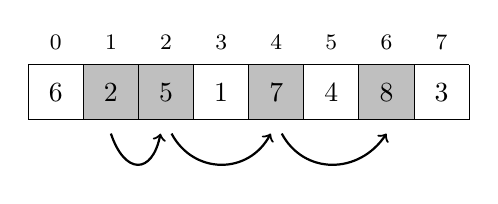
\begin{tikzpicture}[scale=0.7]
\fill[color=lightgray] (1,0) rectangle (2,1);
\fill[color=lightgray] (2,0) rectangle (3,1);
\fill[color=lightgray] (4,0) rectangle (5,1);
\fill[color=lightgray] (6,0) rectangle (7,1);
\draw (0,0) grid (8,1);
\node at (0.5,0.5) {$6$};
\node at (1.5,0.5) {$2$};
\node at (2.5,0.5) {$5$};
\node at (3.5,0.5) {$1$};
\node at (4.5,0.5) {$7$};
\node at (5.5,0.5) {$4$};
\node at (6.5,0.5) {$8$};
\node at (7.5,0.5) {$3$};
\draw[thick,->] (1.5,-0.25) .. controls (1.75,-1.00) and (2.25,-1.00) .. (2.4,-0.25);
\draw[thick,->] (2.6,-0.25) .. controls (3.0,-1.00) and (4.0,-1.00) .. (4.4,-0.25);
\draw[thick,->] (4.6,-0.25) .. controls (5.0,-1.00) and (6.0,-1.00) .. (6.5,-0.25);
\footnotesize
\node at (0.5,1.4) {$0$};
\node at (1.5,1.4) {$1$};
\node at (2.5,1.4) {$2$};
\node at (3.5,1.4) {$3$};
\node at (4.5,1.4) {$4$};
\node at (5.5,1.4) {$5$};
\node at (6.5,1.4) {$6$};
\node at (7.5,1.4) {$7$};
\end{tikzpicture}
\caption{Taulukon pisin nouseva alijono on $[2,5,7,8]$.}
\label{fig:pisnou}
\end{figure}

Voimme lähestyä tehtävää laskemalla jokaiselle taulukon
kohdalle $k=0,1,\dots,n-1$ arvon $\texttt{pisin}(k)$:
kuinka pitkä on pisin nouseva alijono, joka päättyy kohtaan $k$.
Kun olemme laskeneet kaikki nämä arvot, suurin arvoista kertoo meille,
kuinka pitkä on pisin nouseva alijono koko taulukossa.
Esimerkiksi kuvan \ref{fig:pisnou} taulukossa $\texttt{pisin}(6)=4$,
koska kohtaan $6$ päättyvä pisin nouseva alijono on pituudeltaan $4$.

Millainen on sitten pisin kohtaan $k$ päättyvä alijono?
Yksi mahdollisuus on, että alijonossa on vain kohdan $k$ alkio,
jolloin $\texttt{pisin}(k)=1$.
Muussa tapauksessa alijonossa on ensin kohtaan $x$ päättyvä
pisin nouseva alijono, missä $x<k$, ja sitten vielä kohdan $k$ alkio.
Tämä edellyttää, että kohdan $x$ alkio on pienempi
kuin kohdan $k$ alkio.
Tuloksena olevan alijonon pituus on $\texttt{pituus}(x)+1$.
Voimmekin käydä läpi kaikki mahdolliset tavat valita kohta $x$
ja ottaa niistä parhaan vaihtoehdon.

Seuraava koodi laskee jokaiselle $k=0,1,\dots,n-1$
pisimmän kohtaan $k$ päättyvän alijonon pituuden yllä kuvattua
ideaa käyttäen.
Koodi olettaa, että taulukon sisältö on taulukossa \texttt{taulu},
ja se muodostaa taulukon \texttt{pisin}, jossa on pisimpien
alijonojen pituudet.

\begin{code}
for k = 0 to n-1
    pisin[k] = 1
    for x = 0 to k-1
        if taulu[x] < taulu[k] and pisin[x]+1 > pisin[k]
            pisin[k] = pisin[x]+1
\end{code}

Koodin suorituksen jälkeen pisimmän nousevan alijonon pituus on
siis suurin taulukon \texttt{pisin} arvoista.
Tämä algoritmi vie aikaa $O(n^2)$, koska käym\-me jokaisessa
kohdassa $k$ läpi kaikki taulukon edelliset kohdat.

Mitä jos haluaisimme selvittää pisimmän nousevan alijonon
pituuden lisäksi, mistä alkioista se muodostuu?
Tämä onnistuu laajentamalla hieman koodia.
Rakennamme taulukon \texttt{aiempi},
joka kertoo jokaisessa kohdassa, missä on tähän kohtaan
päättyvän pisimmän alijonon edellinen alkio.
Voimme muodostaa taulukon seuraavasti:

\begin{code}
for k = 0 to n-1
    pisin[k] = 1
    aiempi[k] = -1
    for x = 0 to k-1
        if taulu[x] < taulu[k] and pisin[x]+1 > pisin[k]
            pisin[k] = pisin[x]+1
            aiempi[k] = x
\end{code}

Tämän jälkeen jokaisessa kohdassa $k$ arvo $\texttt{aiempi}[k]$
kertoo pisimmän alijonon edellisen alkion kohdan.
Kuitenkin jos alijonon pituus on 1, taulukossa on arvo $-1$.
Voimme nyt selvittää kohtaan $k$ päättyvän alijonon alkiot
käänteisesti seuraavasti:

\begin{code}
while k != -1
    print(taulu[k])
    k = aiempi[k]
\end{code}

Voimme käyttää vastaavaa tekniikkaa
dynaamisessa ohjelmoinnissa aina, kun haluamme
selvittää, mistä aineksista paras ratkaisu muodostuu.

\subsection{Reitti ruudukossa}

Olemme $n \times n$ -ruudukon vasemmassa yläkulmassa ja haluamme
päästä oikeaan alakulmaan.
Jokaisella askeleella voimme siirtyä ruudun alaspäin tai oikealle.
Kuitenkin joissakin ruuduissa on este, emmekä voi kulkea sellaisen
ruudun kautta.
Montako mahdollista reittiä on olemassa?

\begin{figure}
\center
\begin{tikzpicture}[scale=0.7]
\newcommand\ruudukko{
\fill[color=gray] (1,1) rectangle (2,2);
\fill[color=gray] (1,3) rectangle (2,4);
\fill[color=gray] (3,2) rectangle (4,3);
\draw (0,0) grid (4,4);
}
\begin{scope}
\ruudukko
\draw[thick,->,red,line width=2pt] (0.5,3.5) -- (0.5,0.5) -- (3.5,0.5);
\end{scope}
\begin{scope}[xshift=5.5cm]
\ruudukko
\draw[thick,->,red,line width=2pt] (0.5,3.5) -- (0.5,2.5) -- (2.5,2.5) -- (2.5,0.5) -- (3.5,0.5);
\end{scope}
\begin{scope}[xshift=11cm]
\ruudukko
\draw[thick,->,red,line width=2pt] (0.5,3.5) -- (0.5,2.5) -- (2.5,2.5) -- (2.5,1.5) -- (3.5,1.5) -- (3.5,0.5);
\end{scope}
\end{tikzpicture}
\caption{Mahdolliset reitit vasemmasta yläkulmasta oikeaan alakulmaan.}
\label{fig:reiruu}
\end{figure}

Kuvassa \ref{fig:reiruu} on esimerkkitilanne, jossa ruudukon koko on $4 \times 4$.
Tässä tapauksessa meillä on kolme mahdollisuutta, kuinka voimme liikkua
vasemmasta yläkulmasta oikeaan alakulmaan.

Tässä tehtävässä osaongelmat ovat \emph{kaksiulotteisia},
koska olemme reitin joka vaiheessa tietyn rivin tietyllä sarakkeella.
Niinpä määritte\-lemme rekursiivisen funktion, jolla on kaksi
parametria: $\texttt{reitit}(y,x)$ kertoo, montako reittiä on
vasemmasta yläkulmasta ruutuun $(y,x)$.
Tätä funktiota käyttäen $\texttt{reitit}(n,n)$ antaa meille
vastauksen tehtävään.

Hyödyllinen havainto on, että jokaisessa ruudussa meillä on kaksi
mahdollisuutta, kuinka reitti voi tulla ruutuun,
koska voimme tulla joko ylhäältä tai vasemmalta.
Kun haluamme laskea reittien määrää, laskemme yhteen ylhäältä
ja vasemmalta tulevat reitit.
Rajoituksena jos ruudussa on este, siihen tulevien reittien
määrä on aina nolla.

Seuraava koodi toteuttaa dynaamisen ohjelmoinnin:

\begin{code}
reitit[1][1] = 1
for y = 1 to n
    for x = 1 to n
        if este[y][x]
            reitit[y][x] = 0
        else
            reitit[y][x] = reitit[y-1][x]+reitit[y][x-1]
\end{code}

Aluksi merkitsemme muistiin, että vasempaan yläkulmaan on yksi reitti,
koska lähdemme liikkeelle siitä.
Tämän jälkeen laskemme reittien määrän kaikkiin muihin ruutuihin.
Jos ruudussa on este, siihen ei tule mitään reittiä,
ja muuten laskemme yhteen ylhäältä ja vasemmalta tulevat reitit.
Tuloksena on koodi, joka vie aikaa $O(n^2)$.

Huomaa, että tässä käytämme taulukon indeksejä $1,2,\dots,n$
ja oletamme, että indekseissä $0$ on arvona nolla.
Tämä on kätevää, koska meidän ei tarvitse tehdä erikoistapauksia
ruudukon yläreunaa ja vasenta reunaa varten.

\subsection{Repunpakkaus}

Termi \emph{repunpakkaus} viittaa ongelmiin, jossa meillä on joukko
tavaroita, joilla on tietyt painot, 
ja haluamme selvittää, millaisia yhdistelmiä niistä voi muodostaa.
Ongelmasta on monia muunnelmia, joiden yhdistävänä tekijänä on,
että ne voi ratkaista tehokkaasti dynaamisella ohjelmoinnilla.

Seuraavaksi keskitymme ongelmaan, jossa meillä on $n$ tavaraa,
joilla on tietyt painot $p_1,p_2,\dots,p_n$.
Haluamme selvittää kaikki mahdolliset yhteispainot,
jotka voimme muodostaa valitsemalla jonkin osajoukon tavaroista.
Esimerkiksi jos tavaroiden painot ovat $[1,3,3,4]$,
niin mahdolliset yhteispainot ovat $[0,1,3,4,5,6,7,8,10,11]$.
Esimerkiksi yhteispaino $6$ on listalla,
koska saamme sen painoista $3+3=6$,
ja yhteispaino $8$ on listalla,
koska saamme sen painoista $1+3+4=8$.

On helppoa laskea, mikä on suurin mahdollinen tavaroiden yhteispaino,
koska saamme sen valitsemalla kaikki tavarat.
Suurin yhteispaino on siis $s=p_1+p_2+\dots+p_n$.
Tämä on meille hyödyllinen yläraja, koska tiedämme nyt,
että tavaroiden yhteispaino on aina jokin luku välillä $0 \dots s$.

Voimme lähestyä tehtävää dynaamisella ohjelmoinnilla määrittelemällä
funktion $\texttt{painot}(k)$: mitkä kaikki yhteispainot voimme
muodostaa, jos käytös\-sämme on tavarat $1,2,\dots,k$?
Oletamme, että funktio palauttaa \emph{taulukon}, jossa on $s+1$ alkiota:
jokaiselle yhteispainolle $0,1,\dots,s$ tieto siitä,
voimmeko muodostaa sen painoista $p_1,p_2,\dots,p_k$.
Tapaus $\texttt{painot}(0)$ on helppo,
koska kun meillä ei ole mitään tavaroita,
ainoa mahdollinen yhteispaino on $0$.
Tämän jälkeen pystymme laskemaan tapauksen $\texttt{painot}(k)$
ottamalla lähtökohdaksi tapauksen $\texttt{painot}(k-1)$
ja selvittämällä, mitä uusia yhteispainoja voimme muodostaa,
kun saamme käyttää myös painoa $p_k$.

\begin{figure}
\center
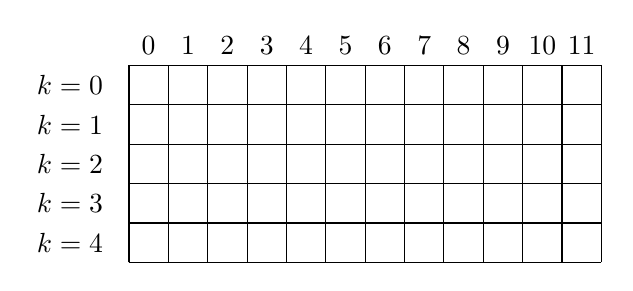
\begin{tikzpicture}[scale=0.5]
\draw (0,0) grid (12,5);
\foreach \x in {0,1,...,11} \node at (\x+0.5,5.5) {\x};
\foreach \y in {0,1,2,3,4} \node at (-1.5,4.5-\y) {$k=\y$};
\foreach \x in {0} \node at (\x+0.5,4.5) {\checkmark};
\foreach \x in {0,1} \node at (\x+0.5,3.5) {\checkmark};
\foreach \x in {0,1,3,4} \node at (\x+0.5,2.5) {\checkmark};
\foreach \x in {0,1,3,4,6,7} \node at (\x+0.5,1.5) {\checkmark};
\foreach \x in {0,1,3,4,5,6,7,8,10,11} \node at (\x+0.5,0.5) {\checkmark};
\end{tikzpicture}
\caption{Mahdolliset yhteispainot, kun painot ovat $[1,3,3,4]$.}
\label{fig:reppak}
\end{figure}

Kuva \ref{fig:reppak} näyttää dynaamisen ohjelmoinnin
taulukoiden sisällön esimerkissämme, jossa painot ovat $[1,3,3,4]$.
Ensimmäisellä rivillä $k=0$, joten ainoa yhteispaino on $0$.
Toisella rivillä $k=1$, joten saamme käyttää painoa $p_1=1$
ja voimme muodostaa yhteispainot $0$ ja $1$.
Kolmannella rivillä $k=2$, jolloin saamme käyttöömme painon $p_2=3$
ja voimme muodostaa yhteispainot $0$, $1$, $3$ ja $4$.
Viimeisellä rivillä käytössämme ovat kaikki painot,
joten se vastaa ongelman ratkaisua.

Voimme toteuttaa dynaamisen ohjelmoinnin kätevästi niin,
että koodissa on vain yksi boolean-taulukko \texttt{reppu},
jossa on $s+1$ alkiota.
Taulukko kertoo laskennan jokaisessa vaiheessa,
mitkä yhteispainot ovat mahdollisia sillä hetkellä.
Aluksi taulukossa kohdassa $0$ on arvo tosi ja
kaikki muut arvot ovat epätosia.
Tämän jälkeen päivitämme taulukkoa lisäämällä mukaan
painoja yksi kerrallaan.

\begin{code}
reppu[0] = true
for i = 1 to n
    for j = s to 0
        if reppu[j]
            reppu[j+p[i]] = true
\end{code}

Laskennan jälkeen voimme tulostaa kaikki
mahdolliset yhteispainot näin:

\begin{code}
for i = 0 to s
    if reppu[i]
        print(i)
\end{code}

Tuloksena olevan algoritmin aikavaativuus on $O(ns)$.
Algoritmin tehokkuus riippuu siis paitsi tavaroiden määrästä,
myös niiden painoista.
Jotta algoritmi on käyttökelpoinen, painojen summan $s$
täytyy olla niin pieni, että voimme varata niin suuren taulukon.

\subsection{Binomikertoimet}

Binomikerroin $\binom{n}{k}$ kertoo, monellako tavalla voimme
muodostaa $n$ alkion joukosta $k$ alkion osajoukon.
Esimerkiksi $\binom{5}{3}=10$, koska voimme muodostaa
joukosta $\{1,2,3,4,5\}$ seuraavat 3 alkion osajoukot:

\begin{multicols}{3}
\begin{itemize}
\item $\{1,2,3\}$
\item $\{1,2,4\}$
\item $\{1,2,5\}$
\item $\{1,3,4\}$
\item $\{1,3,5\}$
\item $\{1,4,5\}$
\item $\{2,3,4\}$
\item $\{2,3,5\}$
\item $\{2,4,5\}$
\item $\{3,4,5\}$
\end{itemize}
\end{multicols}

Binomikerrointen laskemiseen on monia tapoja.
Dynaamisen ohjelmoinnin kannalta kiinnostava tapa on rekursiivinen kaava
\[\binom{n}{k} = \binom{n-1}{k-1} + \binom{n-1}{k}.\]
Kaavassa on ideana, että meillä on kaksi tapaa muodostaa $k$ alkion osajoukko
joukosta $\{1,2,\dots,n\}$.
Jos otamme osajoukkoon mukaan alkion $n$, meidän tulee muodostaa
vielä $k-1$ alkion osajoukko joukosta $\{1,2,\dots,n-1\}$.
Jos taas emme ota osajoukkoon mukaan alkiota $n$, meidän tulee muodostaa
$k$ alkion osajoukko joukosta $\{1,2,\dots,n-1\}$.
Lisäksi pohjatapauksina
\[ \binom{n}{0} = 1,\]
koska voimme muodostaa tyhjän osajoukon yhdellä tavalla, ja
\[ \binom{n}{k} = 0,\,\textrm{jos $k>n$},\]
koska $n$ alkiosta ei voi muodostaa osajoukkoa, jossa on yli $n$ alkiota.

Tämä rekursiivinen kaava tarjoaa meille tavan laskea tehokkaasti
binomikertoimia dynaamisen ohjelmoinnin avulla.
Voimme toteuttaa laskennan seuraavasti:

\begin{code}
for i = 1 to n
    binom[i][0] = 1
    for j = 1 to k
        binom[i][j] = binom[i-1][j-1]+binom[i-1][j]
\end{code}

Koodin suorituksen jälkeen taulukon kohdassa
$\texttt{binom}[n][k]$ on binomikerroin $\binom{n}{k}$.
Algoritmi vie aikaa $O(nk)$, joten sitä voi käyttää
melko suurten binomikerrointen laskemiseen.